\documentclass[8pt,a4paper,landscape,oneside]{amsart}
\usepackage{amsmath, amsthm, amssymb, amsfonts}
\usepackage[T1]{fontenc}
\usepackage[utf8]{inputenc}
\usepackage{booktabs}
\usepackage{caption}
\usepackage{color}
\usepackage{fancyhdr}
\usepackage{float}
\usepackage{fullpage}
\usepackage[top=3pt, bottom=1cm, left=0.3cm, right=0.3cm]{geometry}
\usepackage{graphicx}
\usepackage{subcaption}
\usepackage[scaled]{beramono}
\usepackage{titling}
\usepackage{datetime}
\usepackage{enumitem}
\usepackage{multicol}
\usepackage{lipsum}

\newcommand{\subtitle}[1]{%
  \posttitle{%
    \par\end{center}
    \begin{center}\large#1\end{center}
    \vskip0.1em\vspace{-1em}}%
}

% Minted
\usepackage{minted}
\newcommand{\code}[1]{\inputminted[fontsize=\normalsize,baselinestretch=1]{python}{code/#1}}

% Header/Footer
\pagestyle{fancy}
\lhead{IT-Univerity of Copenhagen}
\rhead{\thepage}
\cfoot{}
\setlength{\headheight}{15.2pt}
\setlength{\droptitle}{-20pt}
\posttitle{\par\end{center}}
\renewcommand{\headrulewidth}{0.4pt}
\renewcommand{\footrulewidth}{0.4pt}

% Math and bit operators
\DeclareMathOperator{\lcm}{lcm}
\newcommand*\BitAnd{\mathrel{\&}}
\newcommand*\BitOr{\mathrel{|}}
\newcommand*\ShiftLeft{\ll}
\newcommand*\ShiftRight{\gg}
\newcommand*\BitNeg{\ensuremath{\mathord{\sim}}}
\DeclareRobustCommand{\stirling}{\genfrac\{\}{0pt}{}}

\newenvironment{myitemize}
{ \begin{itemize}[leftmargin=.5cm]
    \setlength{\itemsep}{0pt}
    \setlength{\parskip}{0pt}
    \setlength{\parsep}{0pt}     }
{ \end{itemize}                  }

% Title/Author
\author{bjal, hefr, krbh}
\title{$\sim$ Python Pirates}
\subtitle{Team Reference Document}
% \date{\ddmmyyyydate{\today{}}}


% Render spaces as middots
\definecolor{middotcolor}{RGB}{180,180,180}
\fvset{showspaces}
\renewcommand\FancyVerbSpace{\textcolor{middotcolor}{·}}

\begin{document}

\begin{figure}
\begin{center}
\vspace{13em}

\includegraphics[]{pythonpiratITUlogo.png}
\end{center}
\end{figure}
\clearpage

\begin{multicols*}{3}
\maketitle
\thispagestyle{fancy}
\vspace{-3em}
\tableofcontents


\section{Common}

    \subsection{Stable matching}
        \code{helloworld.py}
    \subsection{Vertex cover}
        \code{helloworld.py}
    \subsection{Hamiltonian Path}
        \code{helloworld.py}

\section{Graph}

    \subsection{Minimum spanning tree}
    \subsubsection{Kruskal's algorithm}
        \code{kruskal.py}
    \subsubsection{Prim's algorithm}
        \code{prim.py}
    \subsection{Union-Find}
        \code{unionfind.py}
    \subsection{Shortest path}
        \subsubsection{Dijkstra's algorithm}
            \code{djikstra.py}
        \subsubsection{Bellman-Ford} -- Simple Digraph, No negative cycles
            \code{bellmanford.py}
        \subsubsection{Bellman-Ford} -- Multigraph, Possible negative cycles
            \code{bellmanfordgen.py}
    \subsection{Exhastive traversal}
        \subsubsection{Breadth-First Search}
            \code{helloworld.py}
        \subsubsection{Depth-First Search}
            \code{helloworld.py}
    \subsection{Cycles finding}
        \code{helloworld.py}
    \subsection{Flow}
        \subsubsection{Ford-Fulkerson with capacity scaling}
            \code{flow.py}
        \subsubsection{Minimum Cost Maximum Flow using Dijkstra's algorithm}
            \code{helloworld.py}

\section{Strings}

    \subsection{Suffix array}
        \code{helloworld.py}
    \subsection{Knutt-Morris-Pratt}
        \code{helloworld.py}

\section{Geometry}

    \subsection{Closest pair}
        \code{helloworld.py}
    \subsection{Convex hull}
        \code{helloworld.py}
    \subsection{K/D tree}
        \code{helloworld.py}

\section{Search}

    \subsection{Red-Black Binary Search Tree}
        \code{helloworld.py}
    \subsection{Fenwick Tree} -- 1 indexed prefix sums
        \code{fenwick.py}

\section{Combinatorics}

    \subsection{Probability sequences}
        \code{helloworld.py}

\section{Number theory}
    \subsection{Sieve of Eratosthenes - prime generation}
        \code{sieve.py}
    \subsection{Euclidean Algorithm for GCD}
        \code{euclid.py}
    \subsection{Chinese Remainer Theorem}
        \code{chinese_remainder.py}
    \subsection{Chinese Remainer Theorem for non-coprime moduli}
        \code{general_chinese_remainder.py}

\section{Brute force}
    \subsection{Subset enumeration}
        \code{subsets.py}

\section{Mathematics}

    \subsection{Recurrences}
        If $a_n = c_1 a_{n-1} + \dots + c_k a_{n-k}$, and $r_1, \dots, r_k$ are distinct roots of $x^k - c_1 x^{k-1} - \dots - c_k$, there are $d_1, \dots, d_k$ s.t.
        \[a_n = d_1r_1^n + \dots + d_kr_k^n. \]
        Non-distinct roots $r$ become polynomial factors, e.g. $a_n = (d_1n + d_2)r^n$.
        
    \subsection{Sequences}
        \subsubsection{Arithmetic progression}
            Def. $a_n = a + (n-1)d$
            $$ a + ... + z = \frac{n(a+z)}{2}$$
            where $a$: first number, $z$: last number, $n$: amount of numbers
        \subsubsection{Geometric progression}
            $$\sum_{n=0}^{n-1}{ar^k} = ar^0 + ar^1 + ... + ar^{n-1} = a\left(\frac{1-r^n}{1-r}\right)$$
            for $r \neq 1$
        \subsubsection{Triangular numbers}
            $$\sum_{x=1}^{n}{x} = 1 + 2 + 3 + ... + n = \frac{n(n+1)}{2} = \binom{n+1}{2}$$
        \subsubsection{Square pyramidal numbers}
            $$\sum_{x=1}^{n}{x^2} = 1^2 + 2^2 + 3^2 + ... + n^2 = \frac{n(n+1)(2n+1)}{6}$$
        \subsubsection{Harmonic numbers}
            $$\sum_{x=1}^{n}{\frac{1}{x}} = 1 + \frac{1}{2} + \frac{1}{3} + ... + \frac{1}{n} \leq \log_2(N) + 1$$
        \subsubsection{Fibonacci (closed-form)}
            $$\text{fib}(n) = \frac{(1+\sqrt{5})^n - (1-\sqrt{5})^n}{2^n\sqrt{5}}$$
\subsection{Sums}
\[ c^a + c^{a+1} + \dots + c^{b} = \frac{c^{b+1} - c^a}{c-1}, c \neq 1 \]
\begin{align*}
	1 + 2 + 3 + \dots + n &= \frac{n(n+1)}{2} \\
	1^2 + 2^2 + 3^2 + \dots + n^2 &= \frac{n(2n+1)(n+1)}{6} \\
	1^3 + 2^3 + 3^3 + \dots + n^3 &= \frac{n^2(n+1)^2}{4} \\
	1^4 + 2^4 + 3^4 + \dots + n^4 &= \frac{n(n+1)(2n+1)(3n^2 + 3n - 1)}{30} \\
\end{align*}

\subsection{Series}
$$e^x = 1+x+\frac{x^2}{2!}+\frac{x^3}{3!}+\dots,\,(-\infty<x<\infty)$$
$$\ln(1+x) = x-\frac{x^2}{2}+\frac{x^3}{3}-\frac{x^4}{4}+\dots,\,(-1<x\leq1)$$
$$\sqrt{1+x} = 1+\frac{x}{2}-\frac{x^2}{8}+\frac{2x^3}{32}-\frac{5x^4}{128}+\dots,\,(-1\leq x\leq1)$$
$$\sin x = x-\frac{x^3}{3!}+\frac{x^5}{5!}-\frac{x^7}{7!}+\dots,\,(-\infty<x<\infty)$$
$$\cos x = 1-\frac{x^2}{2!}+\frac{x^4}{4!}-\frac{x^6}{6!}+\dots,\,(-\infty<x<\infty)$$

    \subsection{Geometry}
        Geometric areas
    
        Trapezoid area $A = \frac{h}{2} \cdot (a + b)$ where $a$ and $b$ are parallel

        Sphere surface area $S = 4\pi \cdot r^2$
        
        Sphere volume $V = \frac{4}{3} \cdot r^3$
        
        Cone surface $S = \pi r(l+r)$
        
        Cone volume $V = \frac{1}{3}\pi hr^2$

        \subsection{Quadrilaterals}
        With side lengths $a,b,c,d$, diagonals $e, f$, diagonals angle $\theta$, area $A$ and
        magic flux $F=b^2+d^2-a^2-c^2$:
        
        \[ 4A = 2ef \cdot \sin\theta = F\tan\theta = \sqrt{4e^2f^2-F^2} \]
        
         For cyclic quadrilaterals the sum of opposite angles is $180^\circ$,
        $ef = ac + bd$, and $A = \sqrt{(p-a)(p-b)(p-c)(p-d)}$.
        
        
        \subsection{Triangles}
        Side lengths: $a,b,c$\\
        Semiperimeter: $p=\dfrac{a+b+c}{2}$\\
        Area: $A=\sqrt{p(p-a)(p-b)(p-c)}$\\
        Circumradius: $R=\dfrac{abc}{4A}$\\
        Inradius: $r=\dfrac{A}{p}$\\
        Length of median (divides triangle into two equal-area triangles): $m_a=\tfrac{1}{2}\sqrt{2b^2+2c^2-a^2}$\\
        Length of bisector (divides angles in two): $s_a=\sqrt{bc\left[1-\left(\dfrac{a}{b+c}\right)^2\right]}$\\
        Law of sines: $\dfrac{\sin\alpha}{a}=\dfrac{\sin\beta}{b}=\dfrac{\sin\gamma}{c}=\dfrac{1}{2R}$\\
        Law of cosines: $a^2=b^2+c^2-2bc\cos\alpha$\\
        Law of tangents: $\dfrac{a+b}{a-b}=\dfrac{\tan\dfrac{\alpha+\beta}{2}}{\tan\dfrac{\alpha-\beta}{2}}$\\
        

        \subsection{Spherical coordinates}
        \begin{center}
        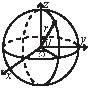
\includegraphics[width=25mm]{sphericalCoordinates}
        \end{center}
        \[\begin{array}{cc}
        x = r\sin\theta\cos\phi & r = \sqrt{x^2+y^2+z^2}\\
        y = r\sin\theta\sin\phi & \theta = \textrm{acos}(z/\sqrt{x^2+y^2+z^2})\\
        z = r\cos\theta & \phi = \textrm{atan2}(y,x)
        \end{array}\]
        

        \subsection{Trigonometry}
        \begin{align*}
        \sin(v+w)&{}=\sin v\cos w+\cos v\sin w\\
        \cos(v+w)&{}=\cos v\cos w-\sin v\sin w\\
        \end{align*}
        \begin{align*}
        \tan(v+w)&{}=\dfrac{\tan v+\tan w}{1-\tan v\tan w}\\
        \sin v+\sin w&{}=2\sin\dfrac{v+w}{2}\cos\dfrac{v-w}{2}\\
        \cos v+\cos w&{}=2\cos\dfrac{v+w}{2}\cos\dfrac{v-w}{2}
        \end{align*}
        \[ (V+W)\tan(v-w)/2{}=(V-W)\tan(v+w)/2 \]
        where $V, W$ are lengths of sides opposite angles $v, w$.
        \begin{align*}
        	a\cos x+b\sin x&=r\cos(x-\phi)\\
        	a\sin x+b\cos x&=r\sin(x+\phi)
        \end{align*}
        where $r=\sqrt{a^2+b^2}, \phi=\operatorname{atan2}(b,a)$.
        

    \subsection{Combinatorics}
        Combinations and Permutations
        
        $P(n,r) = \frac{n!}{(n-r)!}$
        
        $C(n,r) = \binom{n}{r} = \frac{n!}{r!(n-r)!}$
        
        $C(n,r) = C(n, n-r)$

        \subsection{Cycles}
		Let $g_S(n)$ be the number of $n$-permutations whose cycle lengths all belong to the set $S$. Then
		$$\sum_{n=0} ^\infty g_S(n) \frac{x^n}{n!} = \exp\left(\sum_{n\in S} \frac{x^n} {n} \right)$$

	\subsection{Derangements}
		Permutations of a set such that none of the elements appear in their original position.
		\[ \mkern-2mu D(n) = (n-1)(D(n-1)+D(n-2)) = n D(n-1)+(-1)^n = \left\lfloor\frac{n!}{e}\right\rceil \]

	\subsection{Burnside's lemma}
		Given a group $G$ of symmetries and a set $X$, the number of elements of $X$ \emph{up to symmetry} equals
		 \[ {\frac {1}{|G|}}\sum _{{g\in G}}|X^{g}|, \]
		 where $X^{g}$ are the elements fixed by $g$ ($g.x = x$).

		 If $f(n)$ counts ``configurations'' (of some sort) of length $n$, we can ignore rotational symmetry using $G = \mathbb Z_n$ to get
		 \[ g(n) = \frac 1 n \sum_{k=0}^{n-1}{f(\text{gcd}(n, k))} = \frac 1 n \sum_{k|n}{f(k)\phi(n/k)}. \]

\subsection{Partitions and subsets}
	\subsection{Partition function}
		Number of ways of writing $n$ as a sum of positive integers, disregarding the order of the summands.
		\[ p(0) = 1,\ p(n) = \sum_{k \in \mathbb Z \setminus \{0\}}{(-1)^{k+1} p(n - k(3k-1) / 2)} \]
		\[ p(n) \sim 0.145 / n \cdot \exp(2.56 \sqrt{n}) \]

		\begin{center}
		\begin{tabular}{c|c@{\ }c@{\ }c@{\ }c@{\ }c@{\ }c@{\ }c@{\ }c@{\ }c@{\ }c@{\ }c@{\ }c@{\ }c}
			$n$    & 0 & 1 & 2 & 3 & 4 & 5 & 6  & 7  & 8  & 9  & 20  & 50  & 100 \\ \hline
			$p(n)$ & 1 & 1 & 2 & 3 & 5 & 7 & 11 & 15 & 22 & 30 & 627 & $\mathtt{\sim}$2e5 & $\mathtt{\sim}$2e8 \\
		\end{tabular}
		\end{center}

	\subsection{Lucas' Theorem}
		Let $n,m$ be non-negative integers and $p$ a prime. Write $n=n_kp^k+...+n_1p+n_0$ and $m=m_kp^k+...+m_1p+m_0$. Then $\binom{n}{m} \equiv \prod_{i=0}^k\binom{n_i}{m_i} \pmod{p}$.

	\subsection{Binomials}

\subsection{General purpose numbers}
	\subsection{Bernoulli numbers}
		EGF of Bernoulli numbers is $B(t)=\frac{t}{e^t-1}$ (FFT-able).
		$B[0,\ldots] = [1, -\frac{1}{2}, \frac{1}{6}, 0, -\frac{1}{30}, 0, \frac{1}{42}, \ldots]$

		Sums of powers:
		\small
		\[ \sum_{i=1}^n n^m = \frac{1}{m+1} \sum_{k=0}^m \binom{m+1}{k} B_k \cdot (n+1)^{m+1-k} \]
		\normalsize

		Euler-Maclaurin formula for infinite sums:
		\small
		\[ \sum_{i=m}^{\infty} f(i) = \int_m^\infty f(x) dx - \sum_{k=1}^\infty \frac{B_k}{k!}f^{(k-1)}(m) \]
		\[ \approx \int_{m}^\infty f(x)dx + \frac{f(m)}{2} - \frac{f'(m)}{12} + \frac{f'''(m)}{720} + O(f^{(5)}(m)) \]
		\normalsize

	\subsection{Stirling numbers of the first kind}
		Number of permutations on $n$ items with $k$ cycles.
		\begin{align*}
			&c(n,k) = c(n-1,k-1) + (n-1) c(n-1,k),\ c(0,0) = 1 \\
			&\textstyle \sum_{k=0}^n c(n,k)x^k = x(x+1) \dots (x+n-1)
		\end{align*}
		$c(8,k) = 8, 0, 5040, 13068, 13132, 6769, 1960, 322, 28, 1$ \\
		$c(n,2) = 0, 0, 1, 3, 11, 50, 274, 1764, 13068, 109584, \dots$

	\subsection{Eulerian numbers}
		Number of permutations $\pi \in S_n$ in which exactly $k$ elements are greater than the previous element. $k$ $j$:s s.t. $\pi(j)>\pi(j+1)$, $k+1$ $j$:s s.t. $\pi(j)\geq j$, $k$ $j$:s s.t. $\pi(j)>j$.
		$$E(n,k) = (n-k)E(n-1,k-1) + (k+1)E(n-1,k)$$
		$$E(n,0) = E(n,n-1) = 1$$
		$$E(n,k) = \sum_{j=0}^k(-1)^j\binom{n+1}{j}(k+1-j)^n$$

	\subsection{Stirling numbers of the second kind}
		Partitions of $n$ distinct elements into exactly $k$ groups.
		$$S(n,k) = S(n-1,k-1) + k S(n-1,k)$$
		$$S(n,1) = S(n,n) = 1$$
		$$S(n,k) = \frac{1}{k!}\sum_{j=0}^k (-1)^{k-j}\binom{k}{j}j^n$$

	\subsection{Bell numbers}
		Total number of partitions of $n$ distinct elements. $B(n) =$
		$1, 1, 2, 5, 15, 52, 203, 877, 4140, 21147, \dots$. For $p$ prime,
		\[ B(p^m+n)\equiv mB(n)+B(n+1) \pmod{p} \]

	\subsection{Labeled unrooted trees}
		\# on $n$ vertices: $n^{n-2}$ \\
		\# on $k$ existing trees of size $n_i$: $n_1n_2\cdots n_k n^{k-2}$ \\
		\# with degrees $d_i$: $(n-2)! / ((d_1-1)! \cdots (d_n-1)!)$

	\subsection{Catalan numbers}
		\[ C_n=\frac{1}{n+1}\binom{2n}{n}= \binom{2n}{n}-\binom{2n}{n+1} = \frac{(2n)!}{(n+1)!n!} \]
		\[ C_0=1,\ C_{n+1} = \frac{2(2n+1)}{n+2}C_n,\ C_{n+1}=\sum C_iC_{n-i} \]
		${C_n = 1, 1, 2, 5, 14, 42, 132, 429, 1430, 4862, 16796, 58786, \dots}$
		\begin{itemize}[noitemsep]
			\item sub-diagonal monotone paths in an $n\times n$ grid.
			\item strings with $n$ pairs of parenthesis, correctly nested.
			\item binary trees with with $n+1$ leaves (0 or 2 children).
			\item ordered trees with $n+1$ vertices.
			\item ways a convex polygon with $n+2$ sides can be cut into triangles by connecting vertices with straight lines.
			\item permutations of $[n]$ with no 3-term increasing subseq.
		\end{itemize}

    \subsection{Probability} Stochastic variables

        $P(X=r) = C(n,r) \cdot p^r \cdot (1-p)^{n-r}$

        \subsubsection{Bayes' Theorem}

        $P(B|A) = \frac{P(A|B) P(B)}{P(A)}$
        
        $P(B|A) = \frac{P(A|B)P(B)}{P(A|B)P(B) + P(A|\bar{B})P(\bar{B})}$
        
        $P(B_k|A) = \frac{P(A|B_k)P(B_k)}{P(A|B_1)P(B_1) \cdot ... \cdot P(A|B_n)P(B_n)}$

        \subsubsection{Expectation}

        Let $X$ be a discrete random variable with probability $p_X(x)$ of assuming the value $x$. It will then have an expected value (mean) $\mu=\mathbb{E}(X)=\sum_xxp_X(x)$ and variance $\sigma^2=V(X)=\mathbb{E}(X^2)-(\mathbb{E}(X))^2=\sum_x(x-\mathbb{E}(X))^2p_X(x)$ where $\sigma$ is the standard deviation. If $X$ is instead continuous it will have a probability density function $f_X(x)$ and the sums above will instead be integrals with $p_X(x)$ replaced by $f_X(x)$.

Expectation is linear:
\[\mathbb{E}(aX+bY) = a\mathbb{E}(X)+b\mathbb{E}(Y)\]
For independent $X$ and $Y$, \[V(aX+bY) = a^2V(X)+b^2V(Y).\]

    \subsection{Number Theory}
        \subsubsection*{Bezout's Theorem}
        $$
        a,b \in \mathbb{Z^+} \implies \exists s,t \in \mathbb{Z}: \, \gcd(a,b) = sa + tb
        $$
        \subsubsection{Bézout's identity}
	For $a \neq $, $b \neq 0$, then $d=gcd(a,b)$ is the smallest positive integer for which there are integer solutions to
	$$ax+by=d$$
	If $(x,y)$ is one solution, then all solutions are given by
	$$\left(x+\frac{kb}{\gcd(a,b)}, y-\frac{ka}{\gcd(a,b)}\right), \quad k\in\mathbb{Z}$$

        \subsubsection*{Partial Coprime Divisor Property}
        $$
        (\gcd(a,b)=1) \land (a \mid bc) \implies (a \mid c)
        $$
        \subsubsection*{Coprime Modulus Equivalence Property}
        $$
        (\gcd(c,m)=1) \land (ac \equiv bc \mod m) \implies (a \equiv b \mod m)
        $$
        \subsubsection*{Fermat's Little Theorem}
        $$
        (\text{prime}(p)) \land (p \nmid a) \implies (a^{p-1} \equiv 1 \mod p)
        $$
        $$
        (\text{prime}(p)) \implies (a^p \equiv a \mod p) 
        $$


\subsubsection{Pythagorean Triples}
 The Pythagorean triples are uniquely generated by
 \[ a=k\cdot (m^{2}-n^{2}),\ \,b=k\cdot (2mn),\ \,c=k\cdot (m^{2}+n^{2}), \]
 with $m > n > 0$, $k > 0$, $m \bot n$, and either $m$ or $n$ even.

\subsubsection{Primes}
	$p=962592769$ is such that $2^{21} \mid p-1$, which may be useful. For hashing
	use 970592641 (31-bit number), 31443539979727 (45-bit), 3006703054056749
	(52-bit). There are 78498 primes less than 1\,000\,000.

	Primitive roots exist modulo any prime power $p^a$, except for $p = 2, a > 2$, and there are $\phi(\phi(p^a))$ many.
	For $p = 2, a > 2$, the group $\mathbb Z_{2^a}^\times$ is instead isomorphic to $\mathbb Z_2 \times \mathbb Z_{2^{a-2}}$.

\subsubsection{Estimates}
	$\sum_{d|n} d = O(n \log \log n)$.

	The number of divisors of $n$ is at most around 100 for $n < 5e4$, 500 for $n < 1e7$, 2000 for $n < 1e10$, 200\,000 for $n < 1e19$.

\subsubsection{Mobius Function}
\[
	\mu(n) = \begin{cases} 0 & n \textrm{ is not square free}\\ 1 & n \textrm{ has even number of prime factors}\\ -1 & n \textrm{ has odd number of prime factors}\\\end{cases}
\]
  Mobius Inversion:
  \[ g(n) = \sum_{d|n} f(d) \Leftrightarrow f(n) = \sum_{d|n} \mu(d)g(n/d) \]
  Other useful formulas/forms:

  $ \sum_{d | n} \mu(d) = [ n = 1] $ (very useful)

  $ g(n) = \sum_{n|d} f(d) \Leftrightarrow f(n) = \sum_{n|d} \mu(d/n)g(d)$

 $ g(n) = \sum_{1 \leq m \leq n} f(\left\lfloor\frac{n}{m}\right \rfloor ) \Leftrightarrow f(n) = \sum_{1\leq m\leq n} \mu(m)g(\left\lfloor\frac{n}{m}\right\rfloor)$



\subsection{Discrete distributions}

\subsubsection{Binomial distribution}
The number of successes in $n$ independent yes/no experiments, each which yields success with probability $p$ is $\textrm{Bin}(n,p),\,n=1,2,\dots,\, 0\leq p\leq1$.
\[p(k)=\binom{n}{k}p^k(1-p)^{n-k}\]
\[\mu = np,\,\sigma^2=np(1-p)\]
$\textrm{Bin}(n,p)$ is approximately $\textrm{Po}(np)$ for small $p$.

\subsubsection{First success distribution}
The number of trials needed to get the first success in independent yes/no experiments, each wich yields success with probability $p$ is $\textrm{Fs}(p),\,0\leq p\leq1$.
\[p(k)=p(1-p)^{k-1},\,k=1,2,\dots\]
\[\mu = \frac1p,\,\sigma^2=\frac{1-p}{p^2}\]

\subsubsection{Poisson distribution}
The number of events occurring in a fixed period of time $t$ if these events occur with a known average rate $\kappa$ and independently of the time since the last event is $\textrm{Po}(\lambda),\,\lambda=t\kappa$.
\[p(k)=e^{-\lambda}\frac{\lambda^k}{k!}, k=0,1,2,\dots\]
\[\mu=\lambda,\,\sigma^2=\lambda\]

\subsection{Continuous distributions}

\subsubsection{Uniform distribution}
If the probability density function is constant between $a$ and $b$ and 0 elsewhere it is $\textrm{U}(a,b),\,a<b$.
\[f(x) = \left\{
\begin{array}{cl}
\frac{1}{b-a} & a<x<b\\
0 & \textrm{otherwise}
\end{array}\right.\]
\[\mu=\frac{a+b}{2},\,\sigma^2=\frac{(b-a)^2}{12}\]

\subsubsection{Exponential distribution}
The time between events in a Poisson process is $\textrm{Exp}(\lambda),\,\lambda>0$.
\[f(x) = \left\{
\begin{array}{cl}
\lambda e^{-\lambda x} & x\geq0\\
0 & x<0
\end{array}\right.\]
\[\mu=\frac{1}{\lambda},\,\sigma^2=\frac{1}{\lambda^2}\]

\subsubsection{Normal distribution}
Most real random values with mean $\mu$ and variance $\sigma^2$ are well described by $\mathcal{N}(\mu,\sigma^2),\,\sigma>0$.
\[ f(x) = \frac{1}{\sqrt{2\pi\sigma^2}}e^{-\frac{(x-\mu)^2}{2\sigma^2}} \]
If $X_1 \sim \mathcal{N}(\mu_1,\sigma_1^2)$ and $X_2 \sim \mathcal{N}(\mu_2,\sigma_2^2)$ then
\[ aX_1 + bX_2 + c \sim \mathcal{N}(\mu_1+\mu_2+c,a^2\sigma_1^2+b^2\sigma_2^2) \]

\subsection{Markov chains}
A \emph{Markov chain} is a discrete random process with the property that the next state depends only on the current state.
Let $X_1,X_2,\ldots$ be a sequence of random variables generated by the Markov process.
Then there is a transition matrix $\mathbf{P} = (p_{ij})$, with $p_{ij} = \Pr(X_n = i | X_{n-1} = j)$,
and $\mathbf{p}^{(n)} = \mathbf P^n \mathbf p^{(0)}$ is the probability distribution for $X_n$ (i.e., $p^{(n)}_i = \Pr(X_n = i)$),
where $\mathbf{p}^{(0)}$ is the initial distribution.

% \subsubsection{Stationary distribution}
$\mathbf{\pi}$ is a stationary distribution if $\mathbf{\pi} = \mathbf{\pi P}$.
If the Markov chain is \emph{irreducible} (it is possible to get to any state from any state),
then $\pi_i = \frac{1}{\mathbb{E}(T_i)}$ where $\mathbb{E}(T_i)$  is the expected time between two visits in state $i$.
$\pi_j/\pi_i$ is the expected number of visits in state $j$ between two visits in state $i$.

For a connected, undirected and non-bipartite graph, where the transition probability is uniform among all neighbors, $\pi_i$ is proportional to node $i$'s degree.

% \subsubsection{Ergodicity}
A Markov chain is \emph{ergodic} if the asymptotic distribution is independent of the initial distribution.
A finite Markov chain is ergodic iff it is irreducible and \emph{aperiodic} (i.e., the gcd of cycle lengths is 1).
$\lim_{k\rightarrow\infty}\mathbf{P}^k = \mathbf{1}\pi$.

% \subsubsection{Absorption}
A Markov chain is an A-chain if the states can be partitioned into two sets $\mathbf{A}$ and $\mathbf{G}$, such that all states in $\mathbf{A}$ are absorbing ($p_{ii}=1$), and all states in $\mathbf{G}$ leads to an absorbing state in $\mathbf{A}$.
The probability for absorption in state $i\in\mathbf{A}$, when the initial state is $j$, is $a_{ij} = p_{ij}+\sum_{k\in\mathbf{G}} a_{ik}p_{kj}$.
The expected time until absorption, when the initial state is $i$, is $t_i = 1+\sum_{k\in\mathbf{G}}p_{ki}t_k$.

    \subsection{Useful Data Structures in Python}
        \subsubsection{Bit Vector} 
        -- >= 8x more memory efficient bits
            \code{bitvector.py}

    \section{Python3}
    \subsection{Overview}
        \code{python_overview.py}
    \subsection{Standard Library}
        hello
    \subsection{General cheat-sheet}
        \code{python-cheat-sheet.py}
\end{multicols*}

\onecolumn
\begin{multicols*}{3}
    \section{Dump of KTH Stuff}
    \subsection{Overview}
\end{multicols*}

\end{document}